\section{Sets and Operations on Sets} \label{S:setoperations}
%\markboth{Chapter~\ref{C:settheory}. Set Theory}{\ref{S:setoperations}. Operations on Sets}
\setcounter{previewactivity}{0}
%
\begin{previewactivity}[\textbf{Set Operations}]\label{PA:setops} \hfill \\
Before beginning this section, it would be a good idea to review sets and set notation, including the roster method and set builder notation, in Section~\ref{S:predicates}.

In Section~\ref{S:logop}, we used logical operators (conjunction, disjunction, negation) to form new statements from existing statements.  In a similar manner, there are several ways to create new sets from sets that have already been defined.  In fact, we will form these new sets using the logical operators of conjunction (and), disjunction (or), and negation (not).  For example, if the universal set is the set of natural numbers $\N$ and 
\[
A = \{ 1, 2, 3, 4, 5, 6 \} \qquad \text{and} \qquad B = \{ 1, 3, 5, 7, 9 \},
\]
\begin{itemize}
  \item The set consisting of all natural numbers that are in $A$ and are in $B$ is the set $\{1, 3, 5 \}$;
  \item The set consisting of all natural numbers that are in $A$ or are in $B$ is the set 
         $\{ 1, 2, 3, 4, 5, 6, 7, 9 \}$; and
  \item The set consisting of all natural numbers that are in $A$ and are not in $B$ is the set 
         $\{ 2, 4, 6 \}$.
\end{itemize}
These sets are examples of some of the most common set operations, which are given in the following definitions.
\begin{defbox}{intersection}{Let  $A$  and  $B$ be subsets of some universal set  $U$\!.  
The \textbf{intersection}
\index{intersection!of two sets}%
\index{set!intersection}%
of  $A$  and  $B$, written  $A \cap B$ and read ``$A$ intersect $B$,''  is the set of all elements that are in both  $A$  and  $B$.  That is,
\[
A \cap B = \left\{ {x \in U} \mid {x \in A \text{  and  } x \in B}  \right\}\!.
\] 
\label{sym:intersect}
The \textbf{union}
\index{union!of two sets}%
\index{set!union}%
of  $A$  and  $B$, written  $A \cup B$ and read ``$A$ union $B$,'' is the set of all elements that are in  $A$  or in  $B$.  That is,
\[
A \cup B = \left\{ {x \in U} \mid {x \in A \text{  or  } x \in B}  \right\}.
\]} 
\label{sym:union}
\end{defbox}

\begin{defbox}{setdiff}{Let  $A$  and  $B$ be subsets of some universal set  $U$\!.  The 
\textbf{set difference}
\index{difference of two sets}%
\index{set!difference}%
 of  $A$  and  $B$, or \textbf{relative complement}
\index{relative complement}%
\index{set!relative complement}%
 of  $B$  with respect to  $A$, written  $A - B$ and read ``$A$ minus $B$'' or ``the complement of  $B$  with respect to  $A$,'' is the set of all elements in  $A$  that are not in  $B$.  That is,
\[
A - B = \left\{ {x \in U} \mid {x \in A} \text{ and } {x \notin B} \right\}\!.
\] \label{sym:setdiff}
The \textbf{complement}
\index{complement of a set}%
\index{set!complement}%
 of the set  $A$, written  $A^c $ and read ``the complement of $A$,'' is the set of all elements of  $U$  that are not in  $A$.  That is,
\[
A^c  = \left\{ {x \in U} \mid {x \notin A} \right\}\!.
\]} \label{sym:complement}
\end{defbox}

\noindent
For the rest of this \typel activity, the universal set is 
$U = \left\{ {0, 1, 2, 3,  \ldots , 10} \right\}$, and we will use the following subsets of  $U$:
\begin{center}
$A = \left\{ {0, 1, 2, 3, 9} \right\}$ \qquad and \qquad  $B = \left\{ {2, 3, 4, 5, 6} \right\}$.
\end{center}
%Use the roster method to list all of the elements of  $U$  that are in the truth set of each of the following predicates.
So in this case, $A \cap B = \left\{ {x \in U} \mid {x \in A \text{  and  } x \in B}  \right\} = \{2, 3 \}$.  Use the roster method to specify each of the following subsets of $U$.
\begin{multicols}{3}
\begin{enumerate}
%  \item $A \cap B$
  \item $A \cup B$
  \item $A^c$
  \item $B^c$
\end{enumerate}
\end{multicols}

\noindent
We can now use these sets to form even more sets.  For example,
\[
A \cap B^c = \{0, 1, 2, 3, 9 \} \cap \{0, 1, 7, 8, 9, 10 \} = \{0, 1, 9 \}.
\]
Use the roster method to specify each of the following subsets of $U$.
\begin{multicols}{4}
\setcounter{oldenumi}{\theenumi}
\begin{enumerate} \setcounter{enumi}{\theoldenumi}
  \item $A \cup B^c$
  \item $A^c \cap B^c$
  \item $A^c \cup B^c$
  \item $(A \cap B)^c$
\end{enumerate}
\end{multicols}

%  \item $x \in A \text{  and  } x \in B$
%  \item $x \in A \text{  or  } x \in B$
%  \item $x \notin A$
%  \item $x \notin B$
%  \item $x \in A\text{  and  }x \notin B$
%  \item $x \notin A \text{  or  } x \notin B$
%  \item $\mynot  \left( {x \in A\text{  and  }x \in B} \right)$
%  \item $\mynot  \left( {x \in A\text{  or  }x \in B} \right)$
%\end{enumerate}
%\end{multicols}


\end{previewactivity}
\hbreak
\endinput


\begin{previewactivity}[\textbf{Venn Diagrams for Two Sets}]\label{PA:venn} \hfill \\
In \typeu Activity~\ref*{PA:setops}, we worked with verbal and symbolic definitions of set operations.  However, it is also helpful to have a visual representation of sets.  \textbf{Venn diagrams} are used to 
\index{Venn diagram}%
  represent sets by circles (or some other closed geometric shape) drawn inside a rectangle.  The points inside the rectangle represent the universal set  $U$, and the elements of a set are represented by the points inside the circle that represents the set.  For example, Figure~\ref{fig:venn2-prev} is a Venn diagram showing two sets.
\begin{figure}[h]
\begin{center}
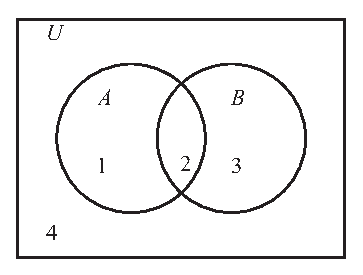
\includegraphics{figps-venn2.eps}
\caption{Venn Diagram for Two Sets} \label{fig:venn2-prev}
\end{center}
\end{figure}

\noindent
In Figure~\ref{fig:venn2-prev}, the elements of  $A$  are represented by the points inside  the left circle, and the elements of  $B$  are represented by the points inside  the right circle.  The four distinct regions in the diagram are numbered for reference purposes only.  (The numbers do not represent elements in a set.)  The following table describes the four regions in the diagram.
$$
\BeginTable
\BeginFormat
| c | l | c |
\EndFormat
" Region  "  Elements of $U$  "   Set  " \\ \_
"1  "  In $A$ and not in $B$  "  $A - B$  " \\
"2  "  In $A$ and in $B$	"  $A \cap B$  " \\
"3  "  In  $B$  and not in $A$  "  $B - A$  " \\
"4  "  Not in $A$ and not in $B$ "	$A^c  \cap B^c $ " \\
\EndTable
$$
We can use these regions to represent other sets.  For example, the set  $A \cup B$  is represented by regions 1, 2, and 3 or the shaded region in Figure~\ref{fig:union2}.
\begin{figure}[h]
\begin{center}
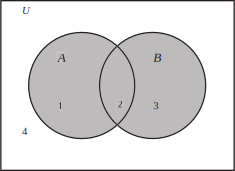
\includegraphics{figps-aunionb.eps}
\caption{Venn Diagram for $A \cup B$} \label{fig:union2}
\end{center}
\end{figure}

\newpage
\noindent
Let $A$ and $B$ be subsets of a universal set $U$.  For each of the following, draw a Venn diagram for two sets and shade the region that represent the specified set.  In addition, describe the set using set builder notation.
\begin{multicols}{3}
\begin{enumerate}
%\item $A \cap B$
\item $A^c$
\item $B^c$
\item $A^c \cup B$
\item $A^c \cup B^c$
\item $\left( A \cap B \right)^c$
\item $\left( A \cup B \right) - \left( A \cap B \right)$
\end{enumerate}
\end{multicols}
\end{previewactivity}
\hbreak
\endinput


%\begin{previewactivity}[Set Equality and Set Containment] \label{PA:setequality} \hfill \\
In Section~\ref{S:predicates}, we considered a set to be any collection of objects that can be thought of as a single entity itself.  We introduced the notation  $y \in A$  to mean, ``$y$ is an element of the set  $A$.''  In addition, we write  $x \notin A$  to mean, ``$x$  is not an element of the set  $A$.''  We also discussed defining sets using the roster method and using set builder notation.

\begin{defbox}{setequality}{
Let $A$ and $B$ be two sets contained in some universal set $U$.  

The sets  $A$  and  $B$ are \textbf{equal}, \label{sym:setequal2} 
\index{equal sets}%
\index{set!equality}%
written  $A = B$, when they have precisely the same elements.  More formally,
\begin{center}
$A = B$ provided that for all $x \in U, x \in A \text{ if and only if } x \in B$.
\end{center}
We write  $A \ne B$ when the two sets  $A$  and  $B$ are not equal.\\

The set  $A$  is a \textbf{subset} of a set  $B$  if each element of  $A$  is an element of 
$B$.  In this case, we write  $A \subseteq B$ and also say that  $A$  is \textbf{contained} \label{sym:subset2}
\index{subset}%
 in  $B$.  More formally,
\begin{center}
$A \subseteq B$ provided that for all $x \in U$, if $x \in A$, then $x \in B$.
\end{center}
When  $A$  is not a subset of  $B$, we write  $A\not  \subseteq B$. \label{sym:notsubset2} \\

The set  $A$  is a \textbf{proper subset} \label{sym:propersub}
\index{proper subset}%
\index{subset!proper}%
of $B$ provided that $A \subseteq B$ and  $A \ne B$.  When $A$ is a proper subset of $B$, we write $A \subset B$.}
\end{defbox}

%\begin{defbox}{setequality}{
%Let $A$ and $B$ be two sets contained in some universal set $U$. The sets  $A$  and  $B$ are \textbf{equal}, 
%\index{equal sets}%
%\index{set!equality}%
%written  $A = B$ \label{sym:setequal}, when they have precisely the same elements.  We write  $A \ne B$ when the two sets  $A$  and  $B$ are not equal.\\
%
%The set  $A$  is \textbf{contained} in a set  $B$  if each element of  $A$  is an element of  $B$.  In this case, we write  $A \subseteq B$ \label{sym:subset} and say that  $A$  is a \textbf{sym:subset}
%\index{subset}%
% of  $B$.  When  $A$  is not a subset of  $B$, we write  $A\not  \subseteq B$ \label{sym:notsubset}.}
%\end{defbox}
%After the preview activities, we will introduce more formal definitions of these concepts that use quantifiers and conditional statements.  These formal definitions will be useful in proofs and forming negations of the definitions.

We will now use the following sets:
\[
\begin{aligned}
A &= \left\{ { - 3, - 2, - 1,0,1,2,3} \right\}  &  B &= \left\{ {\left. {x \in \mathbb{Z}} \right|x^2  < 12} \right\} \\
C &= \left\{ {\left. {x \in \mathbb{Z}} \right|2x - 3 \leq 7} \right\}  &  D &= \left\{ {\left. {y \in \mathbb{Z}} \right|\left| y \right| \leq 5} \right\}   \\
S &= \left\{ {\left. {x \in \mathbb{R}} \right|2x - 3 \leq 7} \right\}  &  T &= \left\{ {\left. {y \in \mathbb{R}} \right|\left| y \right| \leq 5} \right\}  \\
\end{aligned}
\]
%
\begin{enumerate} \item \begin{enumerate}
  \item Write the elements of the set  $B$  using the roster method.
  \item Is the set  $A$   equal to the set  $B$?  Explain.
  \item Is  $A$  a subset of  $B$?  Explain.
  \item Is $A$ a proper subset of $B$?  Explain.
  \item Is  $B$  a subset of  $A$?  Explain.
\end{enumerate}

\item \begin{enumerate} \item Write the elements of the sets  $C$  and  $D$  using the roster method.
  \item Is the set  $C$   equal to the set  $D$?  Explain.
  \item Is  $C$  a subset of  $D$?  Explain.
  \item Is  $D$  a subset of  $C$?  Explain.
  \item Is  $D$  a proper subset of $C$?  Explain.
\end{enumerate}

\item \begin{enumerate} \item Is it possible to write the elements of the sets  $S$  and  $T$  using the roster method?
  \item Is the set  $S$   equal to the set  $T$?  Explain.
  \item Is  $S$  a subset of  $T$?  Explain.
  \item Is  $T$  a subset of  $S$?  Explain.
  \item Is  $T$  a proper subset of $S$?  Explain.
\end{enumerate}

\item The formal definition of ``subset'' states that  $X \subseteq Y$ provided that for all 
$x \in U$, if $x \in X$, then $x \in Y$.  Use this formal definition to complete the following sentence in English:  ``The set  $X$   is not a subset of the set  $Y$ provided that $\ldots$ .''

\end{enumerate}
\end{previewactivity}
\hbreak
%
\begin{previewactivity}[Subsets of a Given Set] \label{PA:subsets} \hfill \\
When a set contains no elements, we say that the set is the \textbf{empty set}.
\index{empty set}%
\index{set!empty}%
The empty set is usually designated by the symbol  $\emptyset $.  For example, the set of all real numbers whose square is equal to $-1$ contains no elements and hence is the empty set.  Using set builder notation, this can be written as 
$\left\{ {x \in \mathbb{R} \mid x^2 = -1} \right\} = \emptyset $.

\begin{enumerate}
\item Let  $A$  be a subset of some universal set  $U$\!.  \label{PA:subsets1}
Are the following statements true or false?  Explain.

  \begin{enumerate}
    \item For all $x \in U$, if  $x \in \emptyset $, then  $x \in A$.
    \item The empty set is a subset of $A$.
  \end{enumerate}

\item Determine all the subsets of the set  $\left\{ a \right\}$. How many subsets does the set  $\left\{ a \right\}$ have?  \label{PA:subsets2}

\item Determine all the subsets of the set  $\left\{ {a, b} \right\}$.  How many subsets does the set  $\left\{ {a, b} \right\}$ have?  \hint  Start with the sets listed in Part~(\ref{PA:subsets2}) and then create the subsets of   $\left\{ {a, b} \right\}$  that are not subsets of   $\left\{ a \right\}$.  \label{PA:subsets3}

\item Determine all the subsets of the set  $\left\{ {a, b, c} \right\}$.  How many subsets does the set  $\left\{ {a, b, c} \right\}$  have?  \hint  Start with the sets listed in Part~(\ref{PA:subsets3}) and then create the subsets of   $\left\{ {a, b, c} \right\}$  that are not subsets of   $\left\{ {a, b} \right\}$.  \label{PA:subsets4}

\item Based on your work in Parts~(\ref{PA:subsets2}), (\ref{PA:subsets3}), and~(\ref{PA:subsets4}), how many subsets do you think a set with  four  elements will have? How many subsets do you think a set with  five  elements will have?  Let  $n \in \mathbb{N}$.  How many subsets do you think a set with  $n$  elements will have?

\end{enumerate}
\end{previewactivity}
\hbreak
%
\begin{previewactivity}[Truth Sets] \label{PA:truthsets} \hfill \\
In Section~\ref{S:predicates}, we studied the truth set of a predicate (open sentence). The \textbf{truth set}
\index{truth set}%
 of a predicate is the collection of objects in the universal set that can be substituted to make the predicate a true statement.  For example,
\begin{itemize}
\item If the universal set is  $\mathbb{R}$, then the truth set of  ``$x^2  - 3x - 10 = 0$''  is  $\left\{ { - 2, 5} \right\}$.

\item If the universal set is  $\mathbb{N}$, then the truth set of  ``$\sqrt n  \in \mathbb{N}$''  is $\left\{ {1, 4, 9, 16,  \ldots } \right\}$.
\end{itemize}
For this activity, the universal set is  $U = \left\{ {0, 1, 2, 3,  \ldots , 10} \right\}$.  We will use the following subsets of  $U$:
\begin{center}
$A = \left\{ {0, 1, 2, 9} \right\}$ \quad and \quad  $B = \left\{ {2, 3, 4, 5, 6} \right\}$.
\end{center}
Use the roster method to list all of the elements of  $U$  that are in the truth set of each of the following predicates.  
%Remember that the connective ``or'' is always used in the inclusive sense.
\begin{multicols}{2}
\begin{enumerate}
  \item $x \in A \text{  and  } x \in B$
  \item $x \in A \text{  or  } x \in B$
  \item $x \notin A$
  \item $x \notin B$
  \item $x \in A\text{  and  }x \notin B$
  \item $x \notin A \text{  or  } x \notin B$
  \item $\mynot  \left( {x \in A\text{  and  }x \in B} \right)$
  \item $\mynot  \left( {x \in A\text{  or  }x \in B} \right)$
\end{enumerate}
\end{multicols}
%\hbreak
\end{previewactivity}

\endinput
 

%
%\subsection*{An Example of Using Set Operations} \label{ss:example-sets}
Following is an example that uses the set operations discussed in Beginning Activity~\ref{PA:setops} where 
we used 
\[
  U = \left\{ {0,1,2,3, \ldots ,10} \right\}\!, \quad  A = \left\{ {0,1,2,9} \right\}\!, \quad  B = \left\{ {2,3,4,5,6} \right\}\!. 
\]
So in this case,

\[
\begin{aligned}
A \cap B &= \left\{ {x \in U \left| {x \in A\text{  and  }x \in B} \right.} \right\} = \left\{ 2 \right\} \\
%  & \\
A \cup B &= \left\{ {x \in U\,\left| {x \in A\text{  or  }x \in B} \right.} \right\} = \left\{ {0,1,2,3,4,5,6,9} \right\} \\
%  &  \\
A^c  &= \left\{ {\left. {x \in U\,} \right|x \notin A} \right\} = \left\{ {3,4,5,6,7,8,10} \right\} \\
%  &  \\
A - B &= \left\{ {\left. {x \in A} \right|x \notin B} \right\} = \left\{ {0,1,9} \right\}\!. \\
\end{aligned}
\]
We can also use these definitions in combinations to form other sets.  For example,
\[
\begin{aligned}
B^c  &= \left\{ {\left. {x \in U} \right|x \notin B} \right\} = \left\{ {0,1,7,8,9,10} \right\} \\
%  &  \\
A^c  \cup  B^c  &= \left\{ {\left. {x \in U} \right|x \in A^c \text{  or  }x \in B^c } \right\} = \left\{ {0,1,3,4,5,6,7,8,9,10} \right\}  \\
%  &  \\
\left( {A \cap B} \right)^c  &= \left\{ {x \in U\left.  \right|x \notin A \cap B} \right\} = \left\{ {0,1,3,4,5,6,7,8,9,10} \right\}\!. \\
\end{aligned}
\]
%
\hbreak
\endinput


\subsection*{Set Equality, Subsets, and Proper Subsets} \label{ss:propersubset} 
In Section~\ref{S:predicates}, we introduced some basic definitions used in set theory, what it means to say that two sets are equal and what it means to say that one set is a subset of another set.  See the definitions on page~\pageref{D:setequality}.  We need one more definition.

\begin{defbox}{propersubset}{
Let $A$ and $B$ be two sets contained in some universal set $U$.  The set  $A$  is a \textbf{proper subset} \label{sym:propersub}
\index{proper subset}%
\index{subset!proper}%
of $B$ provided that $A \subseteq B$ and  $A \ne B$.  When $A$ is a proper subset of $B$, we write $A \subset B$.}
\end{defbox}

  
One reason for the definition of proper subset is that each set is a subset of itself.  That is, 
\begin{center}
If  $A$  is a set, then  $A \subseteq A$.
\end{center}
%
However, sometimes we need to indicate that a set  $X$  is a subset of  $Y$  but  $X \ne Y$. For example, if
\[
X = \left\{ {1, 2} \right\}\text{  and  }Y = \left\{ {0, 1, 2, 3} \right\}\!,
\]
then  $X \subset Y$.  We know that  $X \subseteq Y$ since each element of  $X$  is an element of  $Y$, but  $X \ne Y$ since  $0 \in Y$  and  $0 \notin X$.  (Also, $3 \in Y$  and   $3 \notin X$.)   Notice that the notations  $A \subset B$  and  $A \subseteq B$ are used in a manner similar to inequality notation for numbers ($a < b$  and  $a \leq b$).

It is often very important to be able to describe precisely what it means to say that one set is not a subset of the other.  In the preceding example,  $Y$  is not a subset of  $X$  since there exists an element of $Y$ 
(namely, 0) that is not in $X$.  

In general, the subset relation is described with the use of a universal quantifier since $A \subseteq B$ means that for each element $x$ of $U$, if $x \in A$, then  $x \in B$.   So when we negate this, we use an existential quantifier as follows:
\begin{center}
\begin{tabular}{l l l}
 $A \subseteq B$  &  \qquad means \qquad &  $\left( {\forall x \in U} \right)\left[ {\left( {x \in A} \right) \to \left( {x \in B} \right)} \right]$. \\
  &  &  \\
$A \not\subseteq B$  &  \qquad means \qquad &    $\mynot  \left( {\forall x \in U} \right)\left[ {\left( {x \in A} \right) \to \left( {x \in B} \right)} \right]$  \\
  &  &  $\left( {\exists x \in U} \right) \mynot  \left[ {\left( {x \in A} \right) \to \left( {x \in B} \right)} \right]$ \\
  &  &  $\left( {\exists x \in U} \right)\left[ {\left( {x \in A} \right) \wedge \left( {x \notin B} \right)} \right]$. \\ 
\end{tabular}
\end{center}
So we see that  $A \not\subseteq B$ \label{sym:notsubset2}  means that there exists an  $x$ in $U$  such that  $x \in A$  and  $x \notin B$.

Notice that if $A = \emptyset$, then the conditional statement, ``For each $x \in U$, 
if $x \in \emptyset$, then $x \in B$'' must be true since the hypothesis will always be false.  Another way to look at this is to consider the following statement:

\begin{center}
$\emptyset \not \subseteq B$ means that there exists an $x \in \emptyset$ such that $x \notin B$.
\end{center}
However, this statement must be false since there does not exist an $x$ in $\emptyset$.  Since this is false, we must conclude that $\emptyset \subseteq B$.  Although the facts that $\emptyset \subseteq B$ and $B \subseteq B$ may not seem very important, we will use these facts later, and hence we  summarize them in Theorem~\ref{T:subsets}.

\begin{theorem} \label{T:subsets}
For any set  $B$, $\emptyset  \subseteq B$  and  $B \subseteq B$.  
\end{theorem}

In Section~\ref{S:predicates}, we also defined two sets to be equal when they have precisely the same elements.  For example,
\[
\left\{ {\left. {x \in \mathbb{R}\,} \right|\;x^2  = 4} \right\} = \left\{ { - 2,\;2} \right\}\!.
\]
If the two sets  $A$  and  $B$  are equal, then it must be true that every element of  $A$  is an element of  $B$, that is,  $A \subseteq B$, and it must be true that every element of  $B$  is an element of  $A$, that is, $B \subseteq A$.  Conversely, if  $A \subseteq B$  and   $B \subseteq A$, then  $A$  and  $B$  must have precisely the same elements.  This gives us the following test for set equality:
\begin{theorem} \label{T:setequality}
Let  $A$  and  $B$  be subsets of some universal set  $U$\!.  Then $A = B$  if and only if  $A \subseteq B$  and   $B \subseteq A$.
\end{theorem}

\noindent
%This theorem will provide a useful method for proving that two sets are equal.
\hbreak
\begin{prog}[\textbf{Using Set Notation}] \label{prog:setnotation} \hfill \\
Let the universal set be $U = \left\{ {1,2,3,4,5,6} \right\}$, and let
\[
  A = \left\{ {1,2,4} \right\}\!, \quad  B = \left\{ {1,2,3,5} \right\}\!, \quad   
  C = \left\{ {\left. {x \in U} \right|x^2  \leq 2} \right\}\!. 
\]
In each of the following, fill in the blank with one or more of the symbols  $ \subset, \\ \subseteq, =, \ne, \in ,\text{or } \notin $ so that the resulting statement is true.  For each blank, include all symbols that result in a true statement.  If none of these symbols makes a true statement, write nothing in the blank.
\begin{center}
\begin{tabular}{r p{0.8in} l p{0.5in} r p{0.8in} l }
  $A$   &   & $B$   &   & $\emptyset$   &   & $A$ \\ \cline{2-2} \cline{6-6}
   5    &   & $B$   &   &  $\left\{ 5 \right\}$  & &  $B$ \\ \cline{2-2} \cline{6-6}
  $A$   &   & $C$   &   &  $\left\{ {1,2} \right\}$  &  &  $C$ \\ \cline{2-2} \cline{6-6}
  $\left\{ {1, 2} \right\}$ &  &  $A$ &  &  $\left\{ {4,2,1} \right\}$ & & $A$ \\ \cline{2-2} \cline{6-6}
  6     &  &  $A$ &  &  $B$  &  & $\emptyset$ \\ \cline{2-2} \cline{6-6}
\end{tabular}
\end{center}
\end{prog}
\hbreak

\endinput


\subsection*{More about Venn Diagrams} \label{ss:venn3}
In \typeu Activity~\ref*{PA:venn}, we learned how to use Venn diagrams as a visual representation for sets, set operations, and set relationships.  In that activity, we restricted ourselves to using two sets.  We can, of course, include more than two sets in a Venn diagram.  Figure~\ref{fig:aintersectc} shows a general Venn diagram for three sets (including a shaded region that corresponds to $A \cap C$). 

%\begin{figure}[h!]
%\begin{center}
%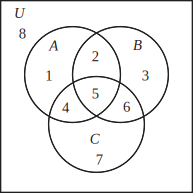
\includegraphics{figps-venn3.eps}
%\caption{Venn Diagram for Three Sets} \label{fig:venn3}
%\end{center}
%\end{figure}

In this diagram, there are eight distinct regions, and each region has a unique reference number.  For example, the set  $A$  is represented by the combination of regions 1, 2, 4, and 5, whereas the set  $C$  is represented by the combination of regions  4, 5, 6, and 7.  This means that the set $A \cap C$ is represented by the combination of regions  4  and  5.  This is shown as the shaded region in Figure~\ref{fig:aintersectc}.

\begin{figure}[h!]
\begin{center}
\scalebox{0.9}{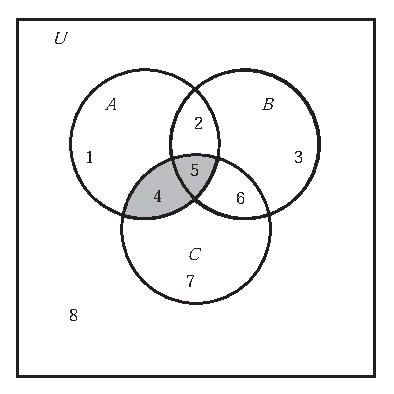
\includegraphics{figps-ainterc3.eps}}
\caption{Venn Diagram for $A \cap C$} \label{fig:aintersectc}
\end{center}
\end{figure}

Finally, Venn diagrams can also be used to illustrate special relationships between sets.  For example, if  $A \subseteq B$, then the circle representing  $A$  should be completely contained in the circle for  $B$.  So if  $A \subseteq B$, and we know nothing about any relationship between the set  $C$ and the sets $A$ and $B$, we could use the Venn diagram shown in Figure~\ref{fig:asubsetb}.

\begin{figure}[h!]
\begin{center}
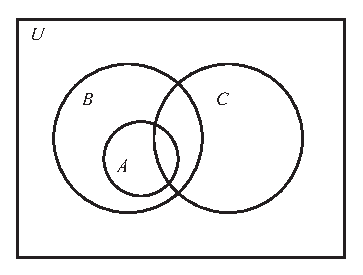
\includegraphics{figps-asubsetb3.eps}
\caption{Venn Diagram Showing $A \subseteq B$} \label{fig:asubsetb}
\end{center}
\end{figure}

\hbreak
\begin{prog}[\textbf{Using Venn Diagrams}] \label{prog:venndiagrams} \hfill \\
Let $A$, $B$, and $C$ be subsets of a universal set $U$.
\begin{enumerate}
  \item For each of the following, draw a Venn diagram for three sets and shade the region(s) that represent the specified set. 
  \begin{multicols}{2}
  \begin{enumerate}
   \item $(A \cap B) \cap C$
   \item $(A \cap B) \cup C$
   \item $\left( A^c \cup B \right)$
   \item $A^c \cap (B \cup C)$
  \end{enumerate}
  \end{multicols}
  \item Draw the most general Venn diagram showing $B \subseteq (A \cup C)$.
  \item Draw the most general Venn diagram showing $A \subseteq \left( B^c \cup C \right)$.
\end{enumerate}
\end{prog}
\hbreak



\endinput
 

\subsection*{The Power Set of a Set}
The symbol  $ \in $  is used to describe a relationship between an element of the universal set and a subset of the universal set, and the symbol  $ \subseteq $  is used to describe a relationship between two subsets of the universal set.  For example, the number 5 is an integer, and so it is appropriate to write  $5 \in \mathbb{Z}$.  It is not appropriate, however, to write  $5 \subseteq \mathbb{Z}$ since 5 is not a set.  It is important to distinguish between 5 and $\left\{ 5 \right\}$.  The difference is that 5 is an integer and $\left\{ 5 \right\}$ is a set consisting of one element.  Consequently, it is appropriate to write  
$\left\{ 5 \right\} \subseteq \mathbb{Z}$, but it is not appropriate to write  
$\left\{ 5 \right\} \in \mathbb{Z}$.  The distinction between these two symbols 
$\left( 5 \text{ and } \left\{ 5 \right\} \right)$ is important when we discuss what is called the power set of a given set.
%
\begin{defbox}{D:powerset}{If  $A$  is a subset of a universal set  $U$, then the set whose members are all the subsets of  $A$  is called the \textbf{power set}
\index{power set}%
\index{set!power}%
 of  $A$.  We denote the power set of  $A$  by  $\mathcal{P}( A )$ 
\label{sym:powerset}.  Symbolically, we write
\[
\mathcal{P}( A ) = \left\{ {X \subseteq U  \mid X \subseteq A} \right\}.
\]
That is,  $X \in \mathcal{P}( A )$  if and  only if  $X \subseteq A$.}
\end{defbox}
When dealing with the power set of  $A$, we must always remember that  $\emptyset  \subseteq A$
and  $A \subseteq A$.  %For reference, we state this as Theorem~\ref{T:subsets}.
%
%\begin{theorem} \label{T:subsets}
%For any set  $A$, $\emptyset  \subseteq A$  and  $A \subseteq A$.  That is,  $\emptyset \in \mathcal{P}\left( A \right)$ and  $A \in \mathcal{P}\left( A \right)$.
%\end{theorem}
%
For example, if  $A = \left\{ {a,b} \right\}$, then the subsets of  $A$  are
\begin{equation} \label{eq:subsets2}
\emptyset,\left\{ a \right\}\!,\left\{ b \right\}\!,\left\{ {a,b} \right\}\!.
\end{equation}
 We can write this as
\[
\mathcal{P}( A ) = \left\{ {\emptyset,\left\{ a \right\}\!,\left\{ b \right\}\!,\left\{ {a,b} \right\}} \right\}\!.
\]
Now let $B = \left\{ {a, b, c} \right\}$.  Notice that $B = A \cup \{ c \}$.  We can determine the subsets of $B$ by starting with the subsets of $A$ in~(\ref{eq:subsets2}).  We can form the other subsets of $B$ by taking the union of each set in~(\ref{eq:subsets2}) with the set $\{c \}$.  This gives us the following subsets of $B$.
\begin{equation} \label{eq:subsets2a}
\{ c \},\left\{ a, c \right\}\!,\left\{ b, c \right\}\!,\left\{ {a,b, c} \right\}\!.
\end{equation}
So the subsets of $B$ are those sets in~(\ref{eq:subsets2}) combined with those sets in~(\ref{eq:subsets2a}).  That is, the subsets of $B$ are
\begin{equation} \label{eq:subsets2b}
\emptyset,\left\{ a \right\}\!,\left\{ b \right\}\!,\left\{ {a,b} \right\}, \{ c \},\left\{ a, c \right\}\!,\left\{ b, c \right\}\!,\left\{ {a,b, c} \right\}\!,
\end{equation}
which means that
\[
\mathcal{P}( B ) = \left\{ {\emptyset,\left\{ a \right\}\!, \left\{ b \right\}\!, \left\{ {a, b} \right\}\!,\left\{ c \right\}\!,\left\{ {a,c} \right\}\!,\left\{ {b,c} \right\}\!,\left\{ {a,b,c} \right\}} \right\}\!.
\]
Notice that we could write
\[
\left\{ {a,c} \right\} \subseteq B \text{  or that  }\left\{ {a,c} \right\} \in \mathcal{P}( B ).
\]
Also, notice that $A$  has two  elements and $A$ has four subsets, and $B$  has  three  elements and $B$  has  eight  subsets.  Now, let  $n$  be a  nonnegative integer.  The following result can be proved using mathematical induction.  (See Exercise~\ref{exer:powerset}.)
\begin{theorem} \label{T:powerset}
Let $n$ be a nonnegative integer and let $T$ be a subset of some universal set.  If the set $T$ has $n$ elements, then the set $T$ has $2^n$ subsets.  That is, $\mathcal{P}(T)$ has $2^n$ elements.
\end{theorem}

\endinput

\subsection*{The Cardinality of a Finite Set}
In our discussion of the power set, we were concerned with the number of elements in a set.  In fact, the number of elements in a finite set is a distinguishing characteristic of the set,  so we give it the following name. 
%
\begin{defbox}{D:cardinality}{The number of elements in a finite set  $A$ is called the \textbf{cardinality}
\index{cardinality}%
\index{cardinality!finite set}%
 of  $A$  and is denoted by  $\card(A)$.} \label{sym:finitecard}
\end{defbox}
%
\noindent
For example,  $\card (\emptyset) = 0$; \qquad	
$\card (\left\{ {a,b} \right\}) = 2$; \qquad	
$\card \left( \mathcal{P}( \left\{ {a,b} \right\}) \right) = 4$.


%\textbf{A Word about Notation:}  We are using the notation  $\left| A \right|$ to denote the cardinality of a set  $A$.  Do not confuse this with the absolute value of a real number.  It is common practice in mathematics to use the same notation for two different concepts when there is little chance of confusion.  We must be careful to use (and understand) the notation in the proper context.  In set theory, $\left| A \right|$ is the cardinality of the set  $A$, and in the algebra of real numbers, $\left| x \right|$ is the absolute value of the real number  $x$.  
\begin{flushleft}
\textbf{Theoretical Note:}  There is a mathematical way to distinguish between finite and infinite sets, and there is a way to define the cardinality of an infinite set.  We will not concern ourselves with this at this time.  More about the cardinality of finite and infinite sets is discussed in Chapter~\ref{C:topicsinsets}.
\end{flushleft}

\endinput

\subsection*{Standard Number Systems}
We can use set notation to specify and help describe our standard number systems.  The starting point is the set of \textbf{natural numbers},
\index{natural numbers}%
 for which we use the roster method.
\[
\N = \left\{ 1, 2, 3, 4, \ldots \;\right\}
\]
The \textbf{integers}
\index{integers}%
 consist of the natural numbers, the negatives of the natural numbers, and zero.  If we let $\N^- = \left\{ \ldots, -4, -3, -2, -1 \right\}$, then we can use set union and write
\[
\Z = \N^- \cup \left\{ 0 \right\} \cup \N.
\]
So we see that $\N \subseteq \Z$, and in fact, $\N \subset \Z$.

We need to use set builder notation for the set $\Q$ of all \textbf{rational numbers}, which consists of quotients of integers.
\[
\Q = \left\{ \left. \frac{m}{n}  \right| m, n \in \Z \text{ and } n \ne 0 \right\}
\]
Since any integer $n$ can be written as $n = \dfrac{n}{1}$, we see that $\Z \subseteq \Q$.  

We do not yet have the tools to give a complete description of the real numbers.
\index{real numbers}%
  We will simply say that the \textbf{real numbers} consist of the rational numbers and the \textbf{irrational numbers}.  In effect, the irrational numbers are the complement of the set of rational numbers $\Q$ in $\R$.  So 
\index{irrational numbers}%
  we can use the notation $\Q^c = \left\{ x \in \R \mid x \notin \Q \right\}$ and write
\[
\R = \Q \cup \Q^c \qquad \text{and} \qquad \Q \cap \Q^c = \emptyset.
\]
A number system that we have not yet discussed is the set of \textbf{complex numbers}.
\index{complex numbers}%
  The complex numbers, $\C$,  consist of all numbers of the form $a + bi$, where $a, b \in \R$ and $i = \sqrt{-1}$ (or $i^2 = -1$).  That is,
\[
\C = \left\{  a + bi \left| \hskip3pt a, b \in \R \text{ and } i = \sqrt{-1} \right. \right\}\!.
\]
We can add and multiply complex numbers as follows:  If $a, b, c, d \in \R$, then
\[
\begin{aligned}
\left( a + bi \right) + \left( c + di \right) &= \left(a + c \right) + \left(b + d \right)i, \text{ and} \\
\left( a + bi \right) \left( c + di \right) &= ac + adi + bci + bdi^2 \\
                                            &= \left(ac - bd \right) + \left(ad + bc \right)i.
\end{aligned}
\]
%\hbreak

\endinput







\hbreak
\endinput


\vskip10pt
\begin{center}
\begin{tabular}{p{0.7in} p{3in}}
 $x \in A$     &	$x$  is an element of the set $A$.  \\  
  \vskip6pt    &   \vskip6pt \\
 $x \notin B$  &  $x$  is not an element of the set  $B$. \\  
  \vskip6pt    &  \vskip6pt \\
 $A=B$         &   The set $A$ \textbf{equals}
\index{equal sets}%
\index{set!equality}%
 the set $B$.  This means that the two sets have precisely the same elements. \\ 
 \vskip6pt     &  \vskip6pt \\
 $\emptyset$   &  The \textbf{empty set}
\index{empty set}%
\index{set!empty}%
 or the set with no elements. \\ 
 \vskip6pt     &  \vskip6pt \\
 $A \subseteq B$  &  The set  $A$  is a \textbf{subset}
\index{subset}%
 of the set $B$ ($A$ is contained in $B$).  This means that each element of $A$ is an element of $B$. \\
 \vskip6pt     &  \vskip6pt \\
 $A \subset B$ &  The set  $A$  is a \textbf{proper subset}
\index{proper subset}%
\index{subset!proper}%
 of $B$.  This means that $A \subseteq B$ and  $A \ne B$.  \\
 \vskip6pt    &  \vskip6pt \\
\end{tabular}
\end{center}







\endinput
